\subsection{بخش ج}
در این بخش به بررسی اثر زاویه دید\LTRfootnote{Look Angle} بر فاصله‌ ازدست‌دهی پرداخته شده است.
\begin{figure}[H]
	\centering
	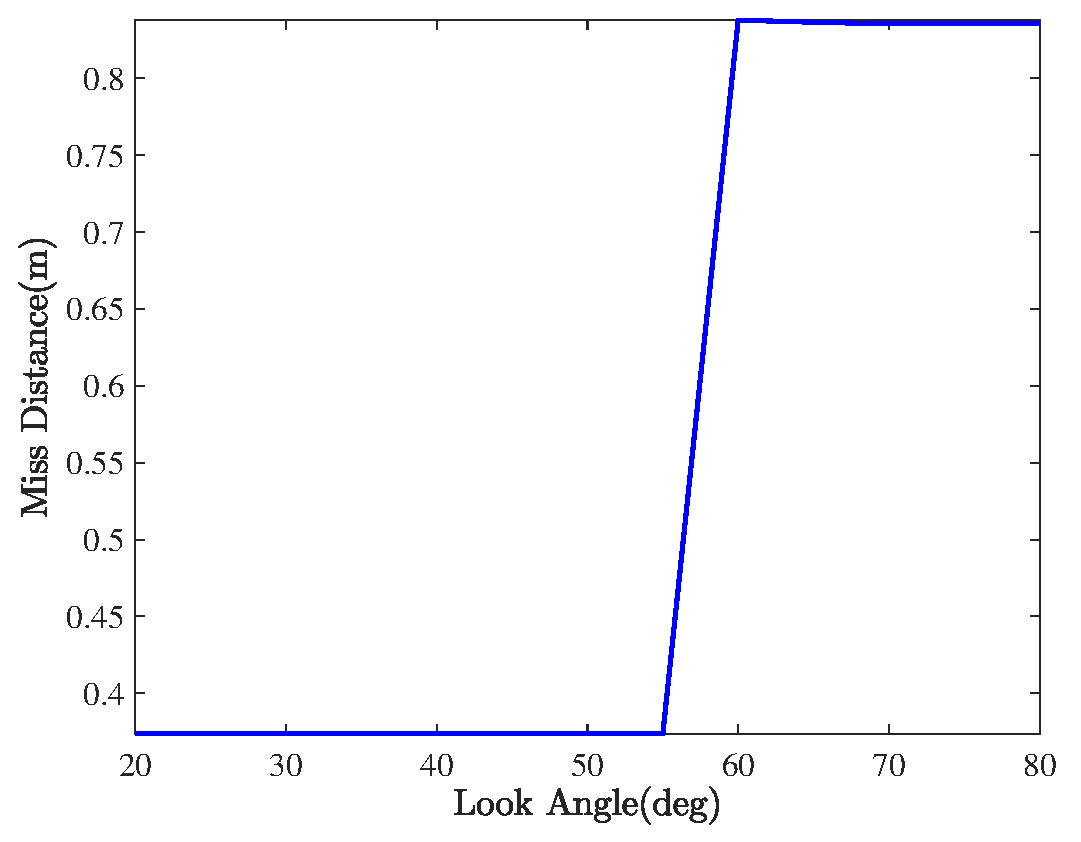
\includegraphics[width=.75\linewidth]{../Figure/Q1/f/MD}
	\caption{فاصله ازدست‌دهی برای مقادیر مختلف زاویه دید}
\end{figure}

با توجه به اینکه شرایط اولیه بر روی مسیر برخورد است بدون فرمان کنترلی نیز به هدف می‌رسد. بنابراین در نبود فرمان بر روی مسیر هدف حرکت کرده و به هدف می‌رسد.